% ----- Presentation -----

\subsection{Presentation}

A \textbf{heuristic algorithm} is a type of algorithm that uses criteria to try to find an approximate solution to a problem, rather than an exact one. Heuristic algorithms are often used when it is not possible to find an ideal solution to a problem, or when a perfect solution would be too time-consuming to compute. They are also used when an approximate solution is good enough. Heuristic algorithms are commonly used in artificial intelligence, computer science, and other fields. They are often used to solve optimization problems, search problems, and other types of problems where an exact solution is not necessary or practical.
\bigskip

A \textbf{constructive heuristic} algorithm is a type of heuristic algorithm that is used to find a solution to a problem by building it incrementally. Constructive heuristics start with a partial solution and gradually improve it until a complete solution is found.
\bigskip

To solve the MEWC with a constructive algorithm, we will need some criteria :

\begin{enumerate}
    \item Add a first Vertex to make a partial solution.
    \item Seek for one of his neighbors. And add it to solution if it's a neighbor of all vertices in solution(to be sure to hold a clique in the final result).
    \item Repeat the step 2 until no vertices is available to add
    \item Calculate the weight of the clique found
\end{enumerate}

We will then have for solution a maximum clique with his weight.
\bigskip

It is important to define the different criteria in a rigorous way.
\bigskip

The first one is the choice of the first Vertex. Indeed, it is this one which will define the quality of our solution. Taking it randomly would be useless and counterproductive for the sake of solving MEWC or for any other problem. There is a lot of implementation which depends on its use. In our project, as it was important, we thought about how to choose it and 2 answers appeared to us, and we have a debate on the subject because we could not reach a consensus on it. We hesitated between these two solutions:

\begin{itemize}
    \item The first idea was to take the highest degree vertex of the graph given as input.
          \begin{itemize}
              \item One reason to choose the highest degree vertex as the first vertex in the solution is that it may be more likely to be part of a maximum edge weight clique(because it's the case where it's the most likely to be member of the biggest clique who could be the MEWC). This is because it will allow more edges to be added to the solution, which can increase the overall sum of edge weights in the clique.
              \item Another reason is that it may be more likely to be connected to other high degree vertices. This means that by adding the highest degree vertex to the clique first, we may be able to include other high degree vertices in the clique as well, which can further increase the overall sum of edge weights.
          \end{itemize}
    \item The second one was to take the vertex with the highest sum of weights of the edges.
          \begin{itemize}
              \item One reason to choose the vertex with the highest edge weight as the first vertex in the clique is that it may be more likely to be part of a maximum edge weight clique(because it's the case where it's the most likely to be member of the most weighted clique who could be the MEWC). This is because adding a vertex with a high edge weight to the clique will contribute more to the overall sum of edge weights in the clique, which is what we are trying to maximize.
              \item Moreover, taking a vertex with higher degree can find adjacent vertices that have lower weight edges, which decreases the probability of finding a maximum weight clique. This does not happen with this choice.
          \end{itemize}
\end{itemize}

\vspace{1\baselineskip}

We will illustrate these explanations with figure \ref{fig:vertex-highest-degree} and \ref{fig:vertex-best-sum-weight-edge} which shows the advantages of each over the other.
\bigskip

\begin{minipage}{\linewidth}
    \begin{minipage}{0.5\textwidth}
        \begin{figure}[H]
            \centering
            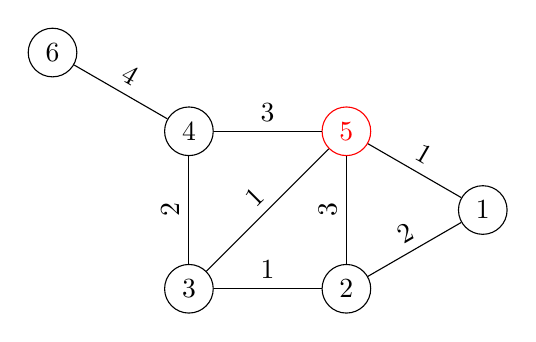
\begin{tikzpicture}[node distance=2cm]
                \node[circle, draw] (1) {1};
                \node[circle, draw] (2) at ([shift=(210:2)] 1) {2};
                \node[circle, draw] (3) [left of=2] {3};
                \node[circle, draw] (4) [above of=3] {4};
                \node[circle, draw, red] (5) [above of=2] {5};
                \node[circle, draw] (6) at ([shift=(150:2)] 4) {6};

                \draw  (1) -- (2) node[midway, above, sloped] {2};
                \draw (1) -- (5) node[midway, above, sloped] {1};
                \draw (2) -- (3) node[midway, above, sloped] {1};
                \draw (2) -- (5) node[midway, above, sloped] {3};
                \draw (3) -- (4) node[midway, above, sloped] {2};
                \draw (4) -- (5) node[midway, above, sloped] {3};
                \draw (4) -- (6) node[midway, above, sloped] {4};
                \draw (5) -- (3) node[midway, above, sloped] {1};
            \end{tikzpicture}
            \caption{Graph illustration for the highest degree vertex}
            \label{fig:vertex-highest-degree}
        \end{figure}
    \end{minipage}
    \begin{minipage}{0.5\textwidth}
        \begin{figure}[H]
            \centering
            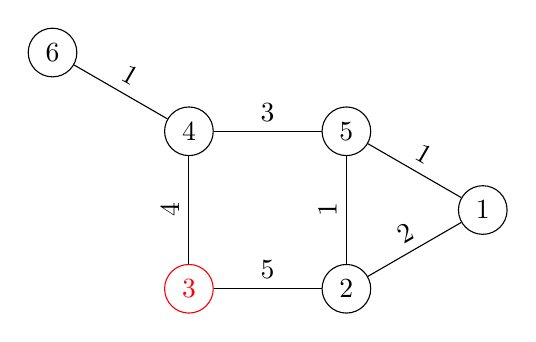
\begin{tikzpicture}[node distance=2cm]
                \node[circle, draw] (1) {1};
                \node[circle, draw] (2) at ([shift=(210:2)] 1) {2};
                \node[circle, draw, red] (3) [left of=2] {3};
                \node[circle, draw] (4) [above of=3] {4};
                \node[circle, draw] (5) [above of=2] {5};
                \node[circle, draw] (6) at ([shift=(150:2)] 4) {6};

                \draw  (1) -- (2) node[midway, above, sloped] {2};
                \draw (1) -- (5) node[midway, above, sloped] {1};
                \draw (2) -- (3) node[midway, above, sloped] {5};
                \draw (2) -- (5) node[midway, above, sloped] {1};
                \draw (3) -- (4) node[midway, above, sloped] {4};
                \draw (4) -- (5) node[midway, above, sloped] {3};
                \draw (4) -- (6) node[midway, above, sloped] {1};
            \end{tikzpicture}
            \caption{Graph illustration for the vertex with the highest sum of weights of the edges}
            \label{fig:vertex-best-sum-weight-edge}
        \end{figure}
    \end{minipage}
\end{minipage}

\vspace{1\baselineskip}

To know which one we were going to use, we implemented both ideas and performed tests on a number of random graphs to see which was the most consistent. For that, we created 10 instances for different number of vertices (from 100 to 1000) and for different connectivity (25 50 75). We applied each of the two algorithms on each instance and averaged the 10 tests to get a usable result. We took the same criterion 2 to homogenize the results (take the vertex which has an adjacent edge with the highest weight compared to the last vertex added in the solution). The following results were obtained. We will name the best sum of adjacent weight $sum$, and the highest degree vertex $degree$.
\bigskip

\begin{figure}[H]
    \centering
    \begin{tikzpicture}
        \begin{semilogyaxis}[
                xlabel = Number of vertices,
                ylabel = Weight of the clique found,
                legend pos = outer north east,
                grid = major,
                width = 0.7\textwidth,
            ]
            \addplot[Blue, dashed, error bars/.cd, y dir=both, y explicit]
            table[x index=0, y index=1] {experiment_data/constructive_sum_alex_25.dat};

            \addplot[Red, dashed, error bars/.cd, y dir=both, y explicit]
            table[x index=0, y index=1] {experiment_data/constructive_sum_alex_50.dat};

            \addplot[Green, dashed, error bars/.cd, y dir=both, y explicit]
            table[x index=0, y index=1] {experiment_data/constructive_sum_alex_75.dat};

            \addplot[Blue, error bars/.cd, y dir=both, y explicit]
            table[x index=0, y index=1] {experiment_data/constructive_degree_alex_25.dat};

            \addplot[Red, error bars/.cd, y dir=both, y explicit]
            table[x index=0, y index=1] {experiment_data/constructive_degree_alex_50.dat};

            \addplot[Green, error bars/.cd, y dir=both, y explicit]
            table[x index=0, y index=1] {experiment_data/constructive_degree_alex_75.dat};

            \addlegendentry{test}

            \legend{sum 25\%, sum 50\%, sum 75\%, degree 25\%, degree 50\%, degree 75\%}
        \end{semilogyaxis}
    \end{tikzpicture}
    \caption{Weight of the clique found for different percentages of connectivity by two criteria algorithm(based on the highest degree/based on the highest sum of the weigh of its adjacent edge)}
    \label{fig:comparaison_degree_sum}
\end{figure}

We can observe in figure \ref{fig:comparaison_degree_sum} that the two results obtained are identical. This can be explained by the fact that on an average of several graphs, the values become more and more regular and homogeneous which does not favor either of the two criteria (while each can be better than the other on some cases). We therefore decided to choose the highest degree vertex because it have less algorithm complexity than its opponent (although both are of the same absolute complexity $\mathcal{O}(n^2)$).
\bigskip

To choose criterion 2, we also considered two implementations. Seek each time for the last vertex added to S its neighbors whose edge is the highest. Or search as done in criterion 1, the highest degree neighbors of the last vertex added to S.
\bigskip

To know which one we were going to use, we implemented both ideas and performed the same process as for choosing criterion 1. The following results were obtained. We will name the neighbors whose edge is the highest $weightN$, and the highest degree neighbors $degreeN$
\bigskip

\begin{figure}[H]
    \centering
    \begin{tikzpicture}
        \begin{semilogyaxis}[
                xlabel = Number of vertices,
                ylabel = Weight of the clique found,
                legend pos = outer north east,
                grid = major,
                width = 0.7\textwidth,
            ]
            \addplot[Blue, dashed, error bars/.cd, y dir=both, y explicit]
            table[x index=0, y index=1] {experiment_data/constructive_degree_alex_25.dat};

            \addplot[Red, dashed, error bars/.cd, y dir=both, y explicit]
            table[x index=0, y index=1] {experiment_data/constructive_degree_alex_50.dat};

            \addplot[Green, dashed, error bars/.cd, y dir=both, y explicit]
            table[x index=0, y index=1] {experiment_data/constructive_degree_alex_75.dat};

            \addplot[Blue, error bars/.cd, y dir=both, y explicit]
            table[x index=0, y index=1] {experiment_data/constructive_degree_youn_25.dat};

            \addplot[Red, error bars/.cd, y dir=both, y explicit]
            table[x index=0, y index=1] {experiment_data/constructive_degree_youn_50.dat};

            \addplot[Green, error bars/.cd, y dir=both, y explicit]
            table[x index=0, y index=1] {experiment_data/constructive_degree_youn_75.dat};

            \addlegendentry{test}

            \legend{weightN 25\%, weightN 50\%, weightN 75\%, degreeN 25\%, degreeN 50\%, degreeN 75\%}
        \end{semilogyaxis}
    \end{tikzpicture}
    \caption{Weight of the clique found for different percentages of connectivity by two criteria of the constructive algorithm (neighbors that share the highest weighted edge/neighbors of the highest degree)}
    \label{fig:comparaison_degreen_weightn}
\end{figure}

We can observe in figure \ref{fig:comparaison_degreen_weightn} that the two results obtained are also identical or present a difference that is not important enough to be noticeable. This can be explained with the same explanation as for the choice of criterion 1. We then chose to take the highest degree neighbors as criterion 2 because its implementation just requires us to make a sorted list of the different vertices of the graph. This makes us gain in constant complexity compared to its opponent.
\bigskip

Constructive heuristic can be contrasted with other types of heuristics, such as local search heuristics, which try to find a solution by making small changes to an existing solution, or random heuristics, which generate solutions randomly and then choose the best one. Constructive heuristics are often used when it is important to find a solution that is complete and comprehensive, rather than just a local improvement.
\bigskip

Examples of some famous problems that are solved using constructive heuristics are the flow shop scheduling, the vehicle routing problem and the open shop problem.

